\documentclass{article}

\usepackage[french]{babel}
\usepackage[utf8]{inputenc}
\usepackage[]{amsmath}
\usepackage{graphicx}
\usepackage{subcaption}
\usepackage{hyperref}

%%%%%%%%%%%%%%%% Lengths %%%%%%%%%%%%%%%%
\setlength{\textwidth}{15.5cm}
\setlength{\evensidemargin}{0.5cm}
\setlength{\oddsidemargin}{0.5cm}

%%%%%%%%%%%%%%%% Variables %%%%%%%%%%%%%%%%
\def\projet{3}
\def\titre{Compression d'image à travers la factorisation SVD}
\def\groupe{4}
\def\equipe{6}
\def\responsible{jeamartinez}
\def\secretary{acattarin}
\def\others{mchellaf, siducamp}

\begin{document}

%%%%%%%%%%%%%%%% Header %%%%%%%%%%%%%%%%
\noindent\begin{minipage}{0.98\textwidth}
  \vskip 0mm
  \noindent
  { \begin{tabular}{p{7.5cm}}
      {\bfseries \sffamily
        Projet \projet} \\ 
      {\itshape \titre}
    \end{tabular}}
  \hfill 
  \fbox{\begin{tabular}{l}
      {~\hfill \bfseries \sffamily Groupe \groupe\ - Equipe \equipe
        \hfill~} \\[2mm] 
      Responsable : \responsible \\
      Secrétaire : \secretary \\
      Codeurs : \others
    \end{tabular}}
  \vskip 4mm ~

  ~~~\parbox{0.95\textwidth}{\small \textit{Résumé~:Le but de ce projet 
  consiste à programmer un algorithme permettant de faire de la compression 
  d'images en utilisant des techniques matricielles basée sur la factorisation SVD.
  Ce type d'algorithme est à relier aux algorithmes de compression avec pertes, 
  dont le plus connu est certainement l'algorithme de compression JPEG, 
  lui-même basé usuellement sur la Discrete Cosine Transform (DCT), une transformation voisine de la transformée de Fourier discrète.} \sffamily }
  \vskip 1mm ~
\end{minipage}

%%%%%%%%%%%%%%%% Main part %%%%%%%%%%%%%%%%
\section{Transformation de Householder}
\label{sec:transfo_householder}

Nous allons en premier lieu mettre en place les fonctions nécessaires à la manipulation de matrices de Householder.
En particulier nous allons créer 3 algorithmes :
\begin{itemize}
  \item householder\_mat(U, V) qui crée la matrice de Householder projetant U sur V
  \item produit\_opti(U, V, vect) qui effectue la multiplication de la matrice de Householder
  $H_{\vec{u},\vec{v}}$ sur le vecteur $vect$ de manière optimisée
  \item produit\_mat\_opti(U, V, M) qui effectue la multiplication de la matrice de Householder
  $H_{\vec{u},\vec{v}}$ sur la matrice $M$ de manière optimisée
\end{itemize}

\subsection{Construction d'une matrice de Householder}
\label{ssec:construc_householder}

\subsection{Application d'une matrice de Householder}
\label{ssec:appli_householder}

Nous allons à présent expliquer la mise au point de l'algorithme produit\_opti(U, V, vect), qui fait la multiplication
$H_{\vec{u},\vec{v}} \cdot vect$ de manière optimisée

Soient deux vecteurs $\vec{u}$ et $\vec{v}$ dont on déduit une matrice de Householder $H_{\vec{u},\vec{v}}$.
Soit un vecteur $\vec{a}$ sur lequel on veut appliquer la matrice de Householder. Les vecteurs sont tous de longueur $n$.

On va utiliser la réécriture $H = I_d - 2 \times N \cdot N^t$ pour écrire un algorithme optimisé de l'application
de $H_{\vec{u},\vec{v}}$.

\begin{align}
  \label{eq:opti_app_hh}
  H_{\vec{u},\vec{v}} \cdot \vec{a} &= (I_d - 2 \times N \cdot N^t) \cdot \vec{a} \\
                                    &= \vec{a} - 2 \times N \cdot N^t \cdot \vec{a} \\
                                    &= \vec{a} - 2 \times N \cdot \underbrace{(N^t \cdot \vec{a})}_{\text{scalaire}} \\
                                    &= \vec{a} - 2 \times \underbrace{(N^t \cdot \vec{a})}_{\text{scalaire}} \cdot N
\end{align}

Alors on peut en déduire un algorithme qui va appliquer directement la matrice $H_{\vec{u},\vec{v}}$ sur $\vec{a}$ à
partir de $\vec{u}$ et $\vec{v}$, et ce en utilisant un unique produit scalaire. Sa complexité est donc en $O(n)$

En utilisant la même relation sur $H_{\vec{u},\vec{v}}$, on peut construire l'algorithme produit\_mat\_opti de manière analogue.

\subsection{Etude de compléxité}
\label{ssec:complex_householder}

Soient une matrice $A$ représentant un ensemble de vecteurs et deux vecteurs $\vec{u}$ et $\vec{v}$ dont
on déduit une matrice de Householder $H_{\vec{u},\vec{v}}$
Appelons $n$ la taille de chacun des vecteurs. \newline

Le produit matriciel entre $H_{\vec{u},\vec{v}}$ et $A$ naïf requiert en premier lieu la construction de 
la matrice de Householder $H_{\vec{u},\vec{v}}$ en brut. L'algorithme construisant la matrice de Householder
effectue une multiplication matrice-vecteur de complexité $O(n^2)$. Par la suite, la multiplication matrice-matrice
entre $H_{\vec{u},\vec{v}}$ et $A$ va demander une complexité $O(n^3)$, en effet l'algorithme fait pour chaque
case $(i,j)$ de la matrice un produit scalaire ligne-colonne de complexité $O(n)$, en sachant que $H_{\vec{u},\vec{v}}$ a $n$ lignes
et colonnes.

Le produit matriciel entre $H_{\vec{u},\vec{v}}$ et $A$ optimisé va utiliser la réécriture de la matrice de Householder :
$H = I_d - 2 \times N \cdot N^t$. 
On va utiliser l'application de la matrice de Householder présentée dans la sous-section \ref{ssec:appli_householder} sur 
chaque vecteur colonne de la matrice $A$, sachant que cette application est en complexité $O(n)$ (un simple produit scalaire).
L'algorithme ne va alors effectuer qu'un produit vectoriel par colonne de la matrice $A$, ce qui nous donne une complexité en $O(n^2)$.

\section{Mise sous forme bidiagonale}
\label{sec:forme_bidiag_}

Afin de transformer une matrice sous la forme SVD, on va d'abord chercher à la bidiagonaliser.
Pour ce faire nous allons utiliser l'algorithme dit de \href[]{https://en.wikipedia.org/wiki/Bidiagonalization}{Golub-Kahan}.

\subsection{Implémentation}
\label{ssec:implem_bidiag_}

L'algorithme consiste à multiplier alternativement la matrice en entrée par des matrices de Householder droites et gauches.
Pour ce faire, on extrait à chaque tour de boucle un vecteur ligne ou colonne de la matrice en entrée pour en déduire une matrice de Householder,
puis on "pad" la matrice de Householder avec en bas à droite le corps de la matrice, en haut à gauche une matrice identité et des 0 aux autres endroits,
comme le montre le schéma \ref{img:pad_HH}.
Cela garantit la préservation de la dimension de la matrice.

\begin{figure}
  \label{img:pad_HH}
  \centering
  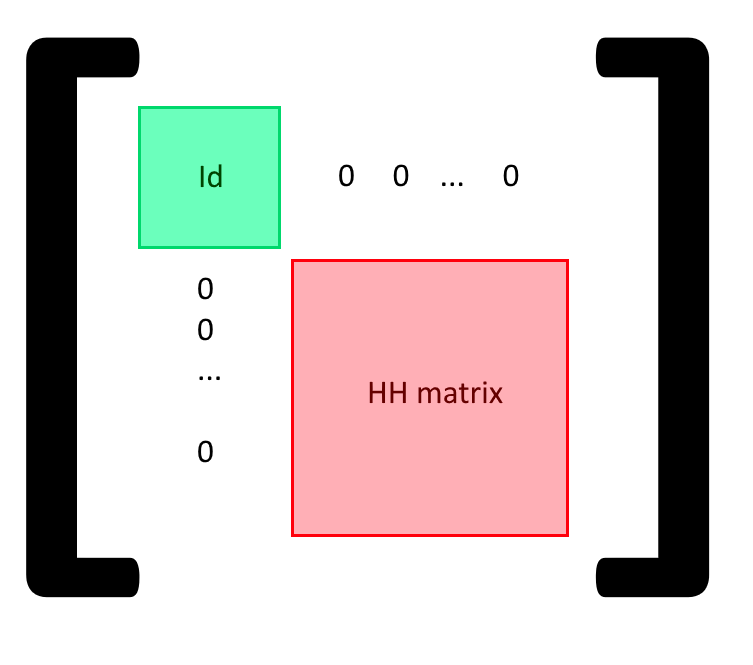
\includegraphics[width=10cm]{../files/hh_padded.png}
\end{figure}

\subsection{Analyse}
\label{ssec:analyse_bidiag}

Nous allons prouver la conservation de l'invariant $Q_{left} \times BD \times Q_{right} = A$ 
à chaque tour de boucle de l'algorithme, à l'aide d'une preuve par induction.

\textbf{Initialisation}: Au début de la première itération de la boucle, 
Qleft et Qright sont tous deux égaux à la matrice identité, et BD est égal à la matrice A. 
Ainsi, $Q_{left} \times BD \times Q_{right} = I_d \times A \times I_d = A$, 
ce qui prouve que l'invariant est vérifié au premier tour de boucle.

\textbf{Hypothèse d'induction}: Supposons que l'invariant est vrai pour une certaine itération i de la boucle,
c'est-à-dire que $Q_{left_i} \times BD_i \times Q_{right_i} = A$, où $Q_{left_i}$, $BD_i$ et $Q_{right_i}$
sont les matrices calculées à la fin de l'itération i.

\textbf{Étape d'induction}: Nous devons montrer que l'invariant est également vrai pour l'itération suivante i+1. 
Pendant cette itération, nous appliquons d'abord une transformation Householder Q1 à la matrice BD pour annuler 
tous les éléments sous la diagonale de la colonne i. Nous mettons à jour Qleft et BD en multipliant par Q1 et Q1 $\times$ BD, respectivement. 
Ensuite, si i n'est pas égal à m-2, nous appliquons une deuxième transformation Householder Q2 à la matrice BD 
pour annuler tous les éléments à droite de la ligne i. Nous mettons à jour Qright et BD en multipliant par Q2 et BD $\times$ Q2, respectivement.

Ainsi, à la fin de l'itération i+1, nous avons:

\begin{itemize}
  \item $BD_{i+1} = Q_{1} \times BD_{i} \times Q_{2}$ si i!=m-2 et $BD_{i+1} = BD_{i}$ sinon
  \item $Q_{left_{i+1}} = Q_{left_{i}} * Q1$
  \item $Q_{right_{i+1}} = Q2 * Q_{right_{i}}$
\end{itemize}

Par conséquent,
\begin{align}
  Q_{left_{i+1}} * BD_{i+1} * Q_{right_{i+1}} &= Q_{left_{i}} * Q_1 * Q_2 * BD_{i} * Q_1 * Q_2 * Q_{right_{i}} \\
                                          &= Q_{left_{i}} * BD_{i} * Q_{right_{i}} \\
                                          &= A
\end{align}


Ainsi, l'invariant est également vrai à l'itération i+1.

Par conséquent, nous pouvons conclure que l'invariant est vrai pour toutes les itérations de la boucle, ce qui signifie que $Q_{left} \times BD \times Q_{right} = A$ à la fin de l'algorithme.
Cette affirmation se vérifie dans les tests grâce à l'algorithme implémenté en Python qui affiche ce produit à chaque tour de boucle.

\section{Transformations QR}
\label{sec:transfo_qr}

\subsection{Implémentation}
\label{ssec:implem_qr}

\subsection{Etude de convergence}
\label{ssec:conv_qr}

\subsection{Analyse}
\label{ssec:analyse_qr}

La matrice $S$ est bidiagonale dès le début de la fonction.

Pour chaque itération de la boucle \verb|for| de la fonction \verb|transfo_qr| :
\smallskip

\noindent La matrice $R1$ est obtenue grâce à une décomposition QR de $S$.

\noindent La matrice $R2$ est obtenue grâce à une décomposition QR de $R2$.

\noindent La matrice $S$ prend les valeurs de $R2$.

\smallskip
Or, la matrice obtenue avec une décomposition QR d'une matrice bidiagonale est également bidiagonale. %à prouver ?

A la première itération, $R1$ est donc bidiagonale (issue de la décomposition QR de $S$). De même, $R2$ est également bidiagonale. Finalement, $S$ prend les valeurs de $R2$. L'invariant est donc vrai après la première itération.

\smallskip

Nous prouvons l'induction exactement de la même manière, puisque nous supposons que $S$ est bidiagonale au début de l'itération.

\subsection{Optimisation pour une matrice bidiagonale}
\label{ssec:opti_bidiag_qr}

\subsection{Mise en forme}
\label{ssec:mise_en_forme_qr}


\section{Application à la compression d'image}
\label{sec:appli_compr_img}

\subsection{Compression}
\label{ssec:compr_img}

\subsection{Analyse quantitative}
\label{ssec:quanti_img}

\subsection{Analyse qualitative}
\label{ssec:quali_img}

\end{document}
